        \documentclass[10pt,a4paper]{article}
        \usepackage{amsmath,amssymb,amsfonts,amscd,graphicx}
        \begin{document}
      consider the following matrix 
      \[
 \mathbf{M}=      \left(\begin{matrix}0 & 1\\-1 & 1\end{matrix}\right)      \]We compute the eigenvalues and the eigenvalues theire multiplicity and the eigenvectors:

\[
\begin{bmatrix}\begin{pmatrix}\frac{1}{2} - \frac{1}{2} \sqrt{3} \mathbf{\imath}, & 1, & \begin{bmatrix}\left(\begin{matrix}- \frac{1}{- \frac{1}{2} + \frac{1}{2} \sqrt{3} \mathbf{\imath}}\\1\end{matrix}\right)\end{bmatrix}\end{pmatrix}, & \begin{pmatrix}\frac{1}{2} + \frac{1}{2} \sqrt{3} \mathbf{\imath}, & 1, & \begin{bmatrix}\left(\begin{matrix}- \frac{1}{- \frac{1}{2} - \frac{1}{2} \sqrt{3} \mathbf{\imath}}\\1\end{matrix}\right)\end{bmatrix}\end{pmatrix}\end{bmatrix}
\]
In detail and with some simplification this means:

\[
\lambda_1=\frac{1}{2} - \frac{1}{2} \sqrt{3} \mathbf{\imath} \hspace{1cm} \lambda_2=\frac{1}{2} + \frac{1}{2} \sqrt{3} \mathbf{\imath}
\]

\[
\mathbf{e_1}=\left(\begin{matrix}\frac{1}{2} \left(1 + \sqrt{3} \mathbf{\imath}\right)\\1\end{matrix}\right) \hspace{1cm} \mathbf{e_2}=\left(\begin{matrix}\frac{1}{2} \left(1 - \sqrt{3} \mathbf{\imath}\right)\\1\end{matrix}\right)
\]
Now we can write down two independent solutions
\[
\mathbf{s_1}(t)=e^{\lambda_1 t}\mathbf{e_1}=\left(\begin{matrix}\mathbf{\imath} \left(- \frac{1}{2} e^{\frac{1}{2} t} \sin{\left (\frac{1}{2} \sqrt{3} t \right )} + \frac{1}{2} \sqrt{3} e^{\frac{1}{2} t} \cos{\left (\frac{1}{2} \sqrt{3} t \right )}\right) + \frac{1}{2} \sqrt{3} e^{\frac{1}{2} t} \sin{\left (\frac{1}{2} \sqrt{3} t \right )} + \frac{1}{2} e^{\frac{1}{2} t} \cos{\left (\frac{1}{2} \sqrt{3} t \right )}\\- \mathbf{\imath} e^{\frac{1}{2} t} \sin{\left (\frac{1}{2} \sqrt{3} t \right )} + e^{\frac{1}{2} t} \cos{\left (\frac{1}{2} \sqrt{3} t \right )}\end{matrix}\right)
\]

\[
\mathbf{s_2}(t)=e^{\lambda_2 t}\mathbf{e_2}=\left(\begin{matrix}\mathbf{\imath} \left(\frac{1}{2} e^{\frac{1}{2} t} \sin{\left (\frac{1}{2} \sqrt{3} t \right )} - \frac{1}{2} \sqrt{3} e^{\frac{1}{2} t} \cos{\left (\frac{1}{2} \sqrt{3} t \right )}\right) + \frac{1}{2} \sqrt{3} e^{\frac{1}{2} t} \sin{\left (\frac{1}{2} \sqrt{3} t \right )} + \frac{1}{2} e^{\frac{1}{2} t} \cos{\left (\frac{1}{2} \sqrt{3} t \right )}\\\mathbf{\imath} e^{\frac{1}{2} t} \sin{\left (\frac{1}{2} \sqrt{3} t \right )} + e^{\frac{1}{2} t} \cos{\left (\frac{1}{2} \sqrt{3} t \right )}\end{matrix}\right)
\]
where we applied the euler formula and ordered for real and imaginary parts. From this representation it is obvious that these solutions are conjugent to each other. This suggests the following way to construct two real valued solutions as linear combinations of $ \mathbf{s_1} $ and $ \mathbf{s_2} $.
\[
\mathbf{n_1}(t)=  \mathbf{s_2}(t)+\mathbf{s_2}(t) =\left(\begin{matrix}\left(\sqrt{3} \sin{\left (\frac{1}{2} \sqrt{3} t \right )} + \cos{\left (\frac{1}{2} \sqrt{3} t \right )}\right) e^{\frac{1}{2} t}\\2 e^{\frac{1}{2} t} \cos{\left (\frac{1}{2} \sqrt{3} t \right )}\end{matrix}\right)
\]

\[
\mathbf{n_2}(t)=i(\mathbf{s_2}(t)-\mathbf{s_2}(t))=\left(\begin{matrix}\left(\sin{\left (\frac{1}{2} \sqrt{3} t \right )} - \sqrt{3} \cos{\left (\frac{1}{2} \sqrt{3} t \right )}\right) e^{\frac{1}{2} t}\\2 e^{\frac{1}{2} t} \sin{\left (\frac{1}{2} \sqrt{3} t \right )}\end{matrix}\right)
\]
We can now express any solution either in terms of $ \mathbf{s_1} $ and $ \mathbf{s_2} $ or $ \mathbf{n_1} $ and $ \mathbf{n_2} $. We will now proceed to do so for a solution that matches an arbitrary real start vector. We look for a set of (real) constants $\{r_1,r_2\} $ that fulfills the following equation:
\[
\left(\begin{matrix}x_{0}\\y_{0}\end{matrix}\right)=\left(\begin{matrix}3\\-5\end{matrix}\right)=r_1 \mathbf{n_1}(0)+ r_2 \mathbf{n_2}(0)=r_1 \left(\begin{matrix}1\\2\end{matrix}\right) r_2 \left(\begin{matrix}- \sqrt{3}\\0\end{matrix}\right)
\]
So we have to solve the linear system:
\[
\left(\begin{matrix}3\\-5\end{matrix}\right)=\left(\begin{matrix}1 & - \sqrt{3}\\2 & 0\end{matrix}\right) \left(\begin{matrix}r_{1}\\r_{2}\end{matrix}\right)
\]
The Solution is: \[ \left(\begin{matrix}r_{1}\\r_{2}\end{matrix}\right)=\left(\begin{matrix}- \frac{5}{2}\\- \frac{11}{6} \sqrt{3}\end{matrix}\right) \]We can now plot the solution.\begin{figure}[t]
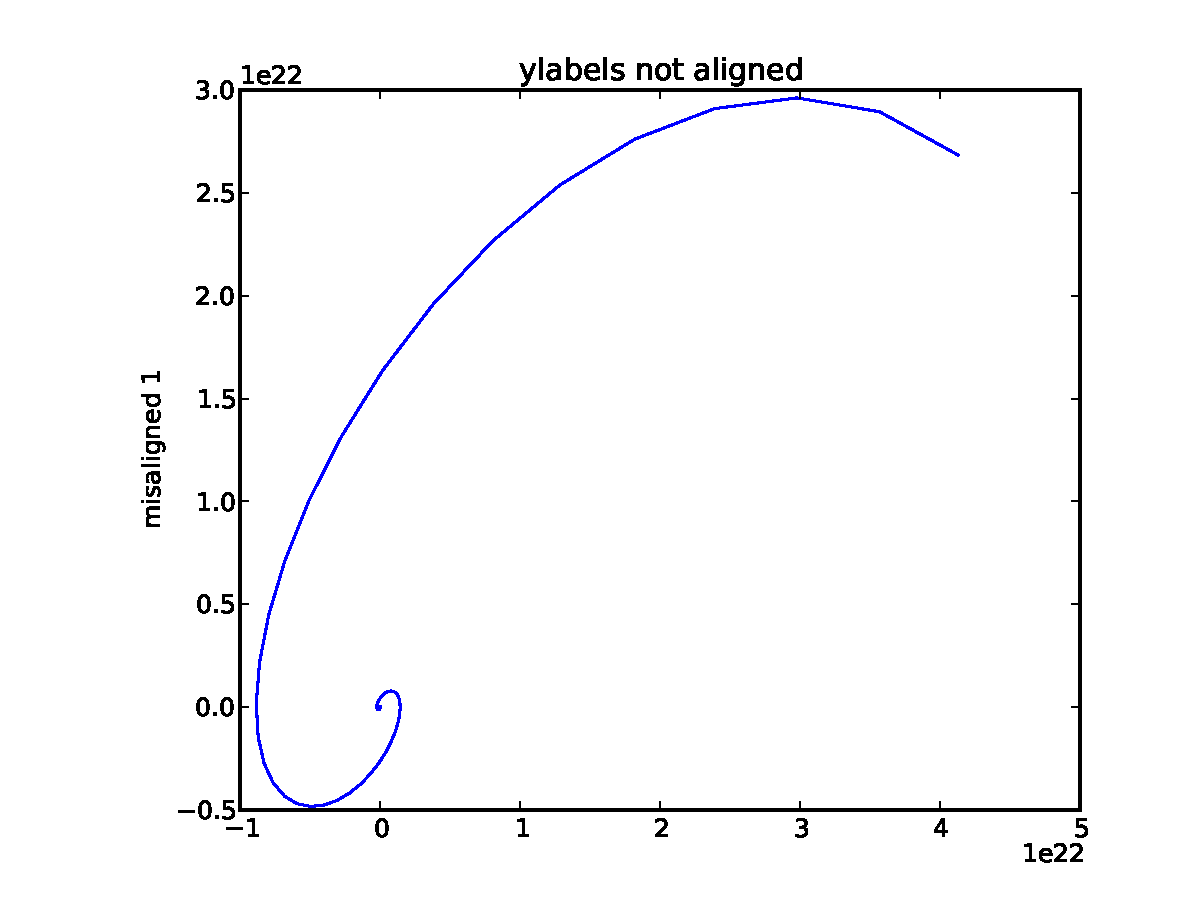
\includegraphics[width=12cm]{myfile}
\caption{TEXT}
\end{figure}
\end{document}